\documentclass[10pt]{beamer}
\usepackage[magyar]{babel}
\usepackage[utf8]{inputenc}
\usepackage{t1enc}
\usepackage{wrapfig}
\usetheme[pageofpages=/,alternativetitlepage=true,]{Torino}
\usecolortheme{freewilly}
\usepackage{mathtools}

\author{Olar Alex}
\title{A CBM/FAIR szimuláció használata és részecske klaszterezés nehézion ütközésekben}
\institute{Eötvös Loránd Tudományegyetem \\ \scriptsize{Fizika BSc III.}}
\date{Kari TDK Konferencia 2017. december 9.}


\begin{document}
\begin{frame}[t,plain]
\titlepage
\end{frame}

\begin{frame}[t]{Vázlat}
\begin{itemize}
\item QCD a CBM-ben
\item A CBM detektor
\item Mini projekt: $\Phi$-mezon
\item A szimulációs program
\item Nehézion fizika itthon
\item Részecske klaszterezés - MST (/ BFS)
\item Hivatkozások
\end{itemize}
\end{frame}

\begin{frame}[t]{QCD a CBM-ben}
\begin{figure}[H!]
\centering
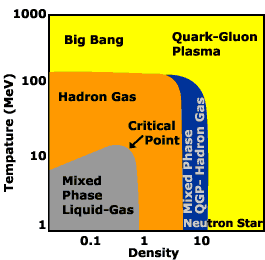
\includegraphics[width=0.6\textwidth]{../latex/cbm_phase1.png}
\end{figure}
\end{frame}

\begin{frame}[t]{QCD a CBM-ben}
\begin{figure}[H!]
\centering
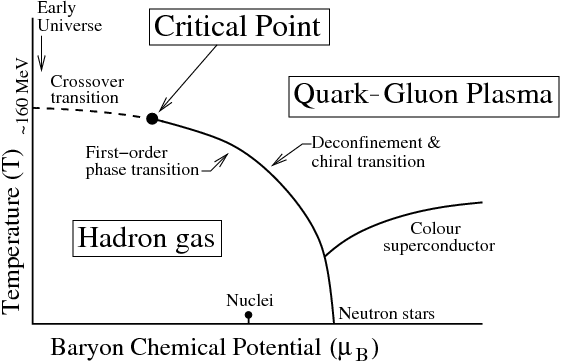
\includegraphics[width=0.84\textwidth]{../latex/CBM_phase_trans.png}
\end{figure}
\end{frame}

\begin{frame}[t]{A CBM detektor}
\begin{figure}[H!]
\centering
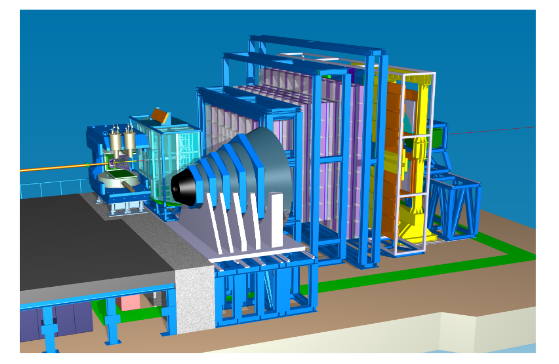
\includegraphics[width=0.84\textwidth]{../latex/cbm_detector.png}
\end{figure}
\end{frame}

\begin{frame}[t]{$\Phi$-mezon}
\begin{minipage}{\textwidth}
\begin{minipage}{0.48\textwidth}
\begin{figure}[H!]
\centering
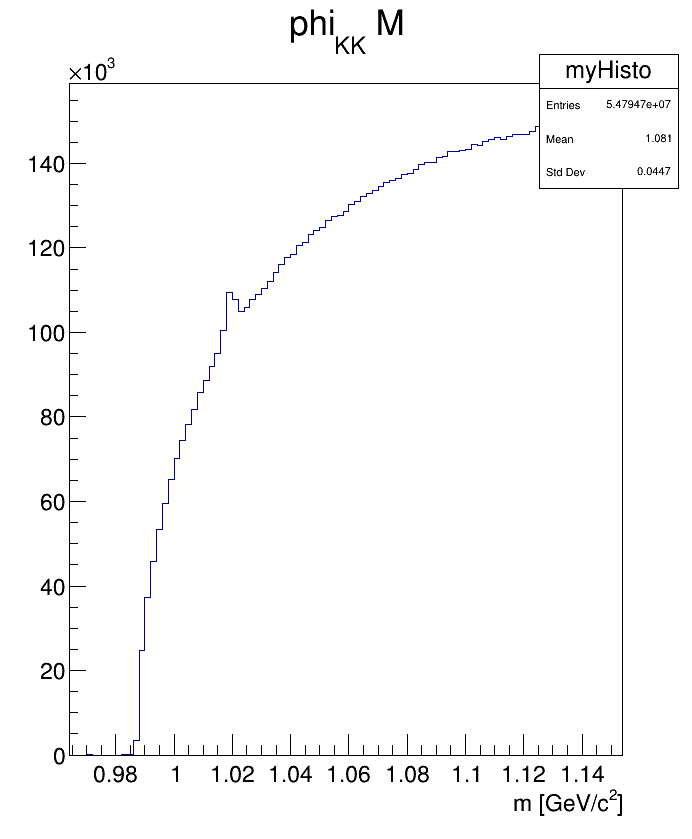
\includegraphics[width=0.94\textwidth]{../latex/phi_KK_Mzoom.png}
\end{figure}
\end{minipage}
\begin{minipage}{0.45\textwidth}
\centering
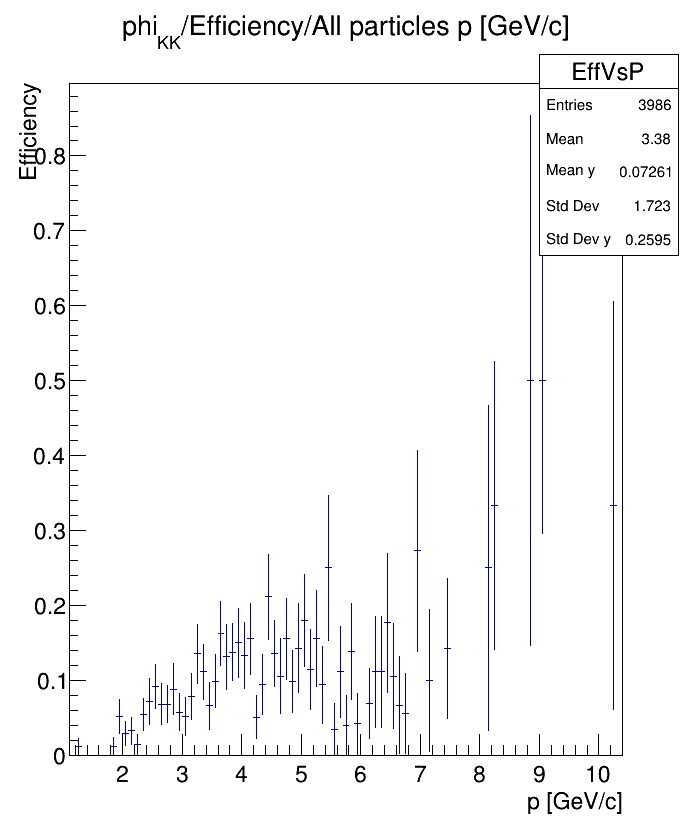
\includegraphics[width=0.97\textwidth]{../latex/efficieny.png}
\end{minipage}
\end{minipage}
\end{frame}

\begin{frame}[t]{A szimulációs program}
\begin{minipage}{\textwidth}
\begin{minipage}{0.78\textwidth}
\begin{figure}[H!]
\centering
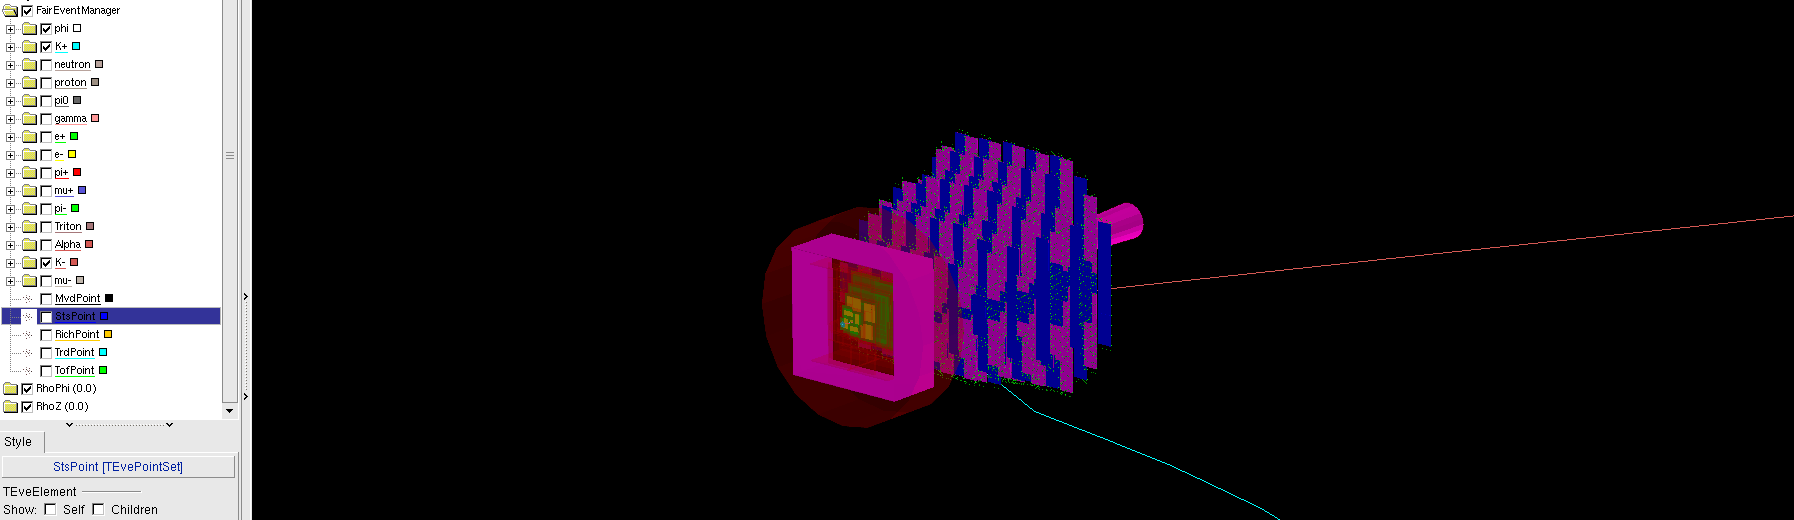
\includegraphics[width=0.94\textwidth]{../latex/k-k+decayofphi.png}
\end{figure}
\end{minipage}
\begin{minipage}{0.72\textwidth}
\centering
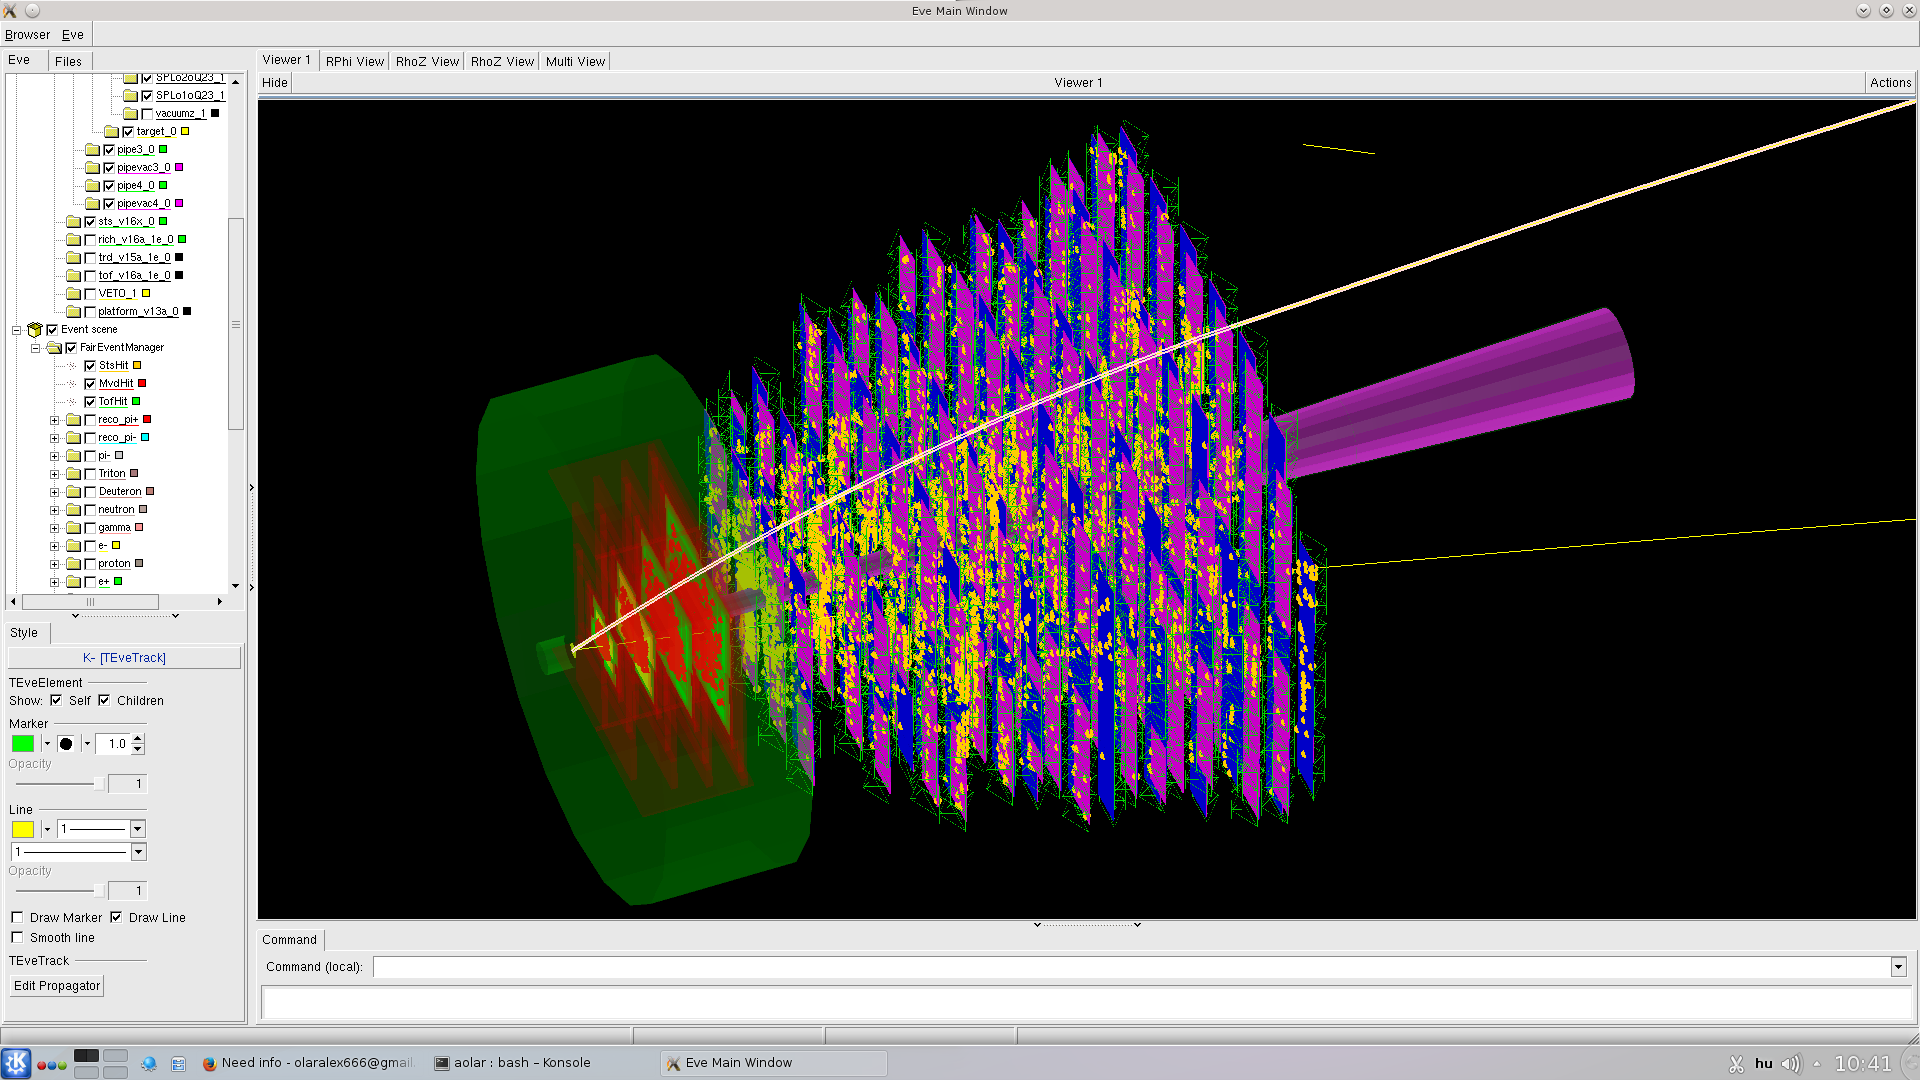
\includegraphics[width=0.97\textwidth]{../latex/reco2.png}
\end{minipage}
\end{minipage}
\end{frame}

\begin{frame}[t]{Nehézion fizika itthon - Részecske klaszterezés - MST}
\centering
\begin{minipage}{\textwidth}
\begin{minipage}{0.48\textwidth}
\centering
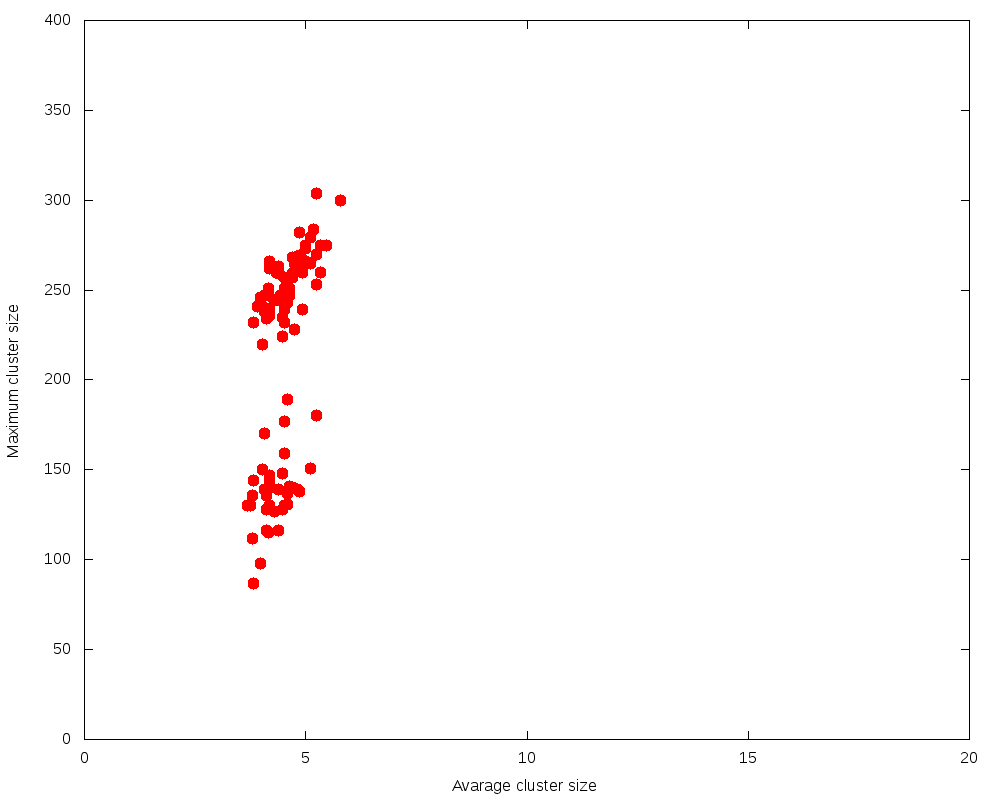
\includegraphics[width=0.94\textwidth]{../latex/mean-max18_120.png}
\end{minipage}
\begin{minipage}{0.48\textwidth}
\centering
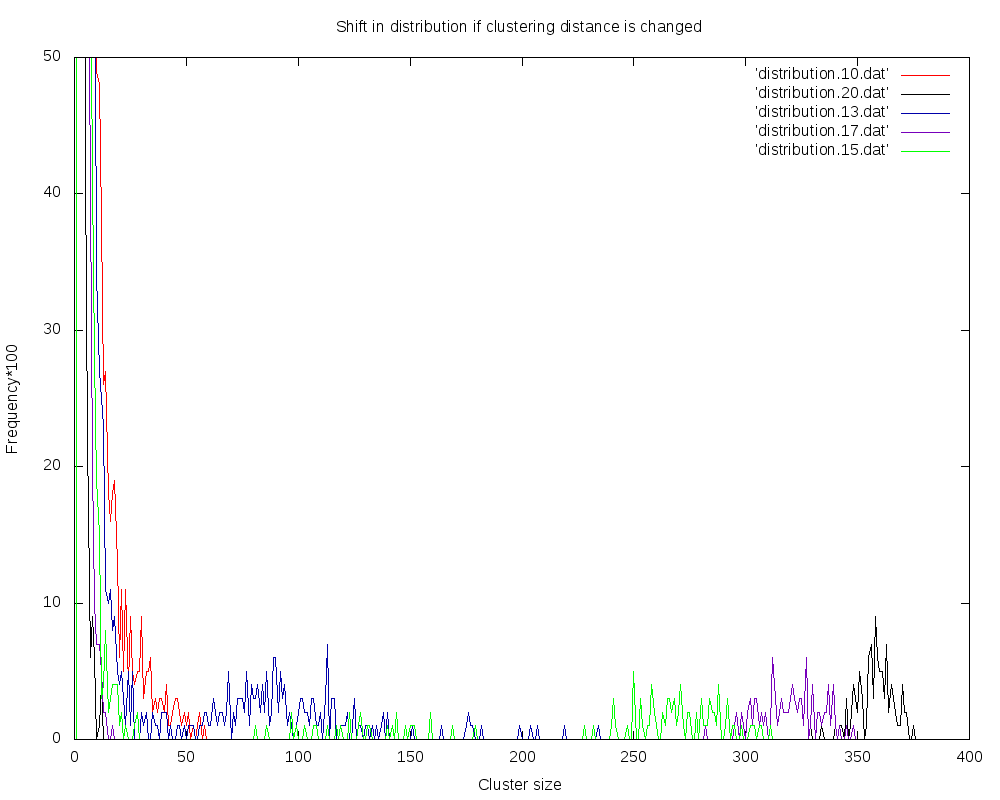
\includegraphics[width=0.94\textwidth]{../latex/ShiftInDistro100.png}
\end{minipage}
\end{minipage}
\begin{minipage}{0.45\textwidth}
\centering
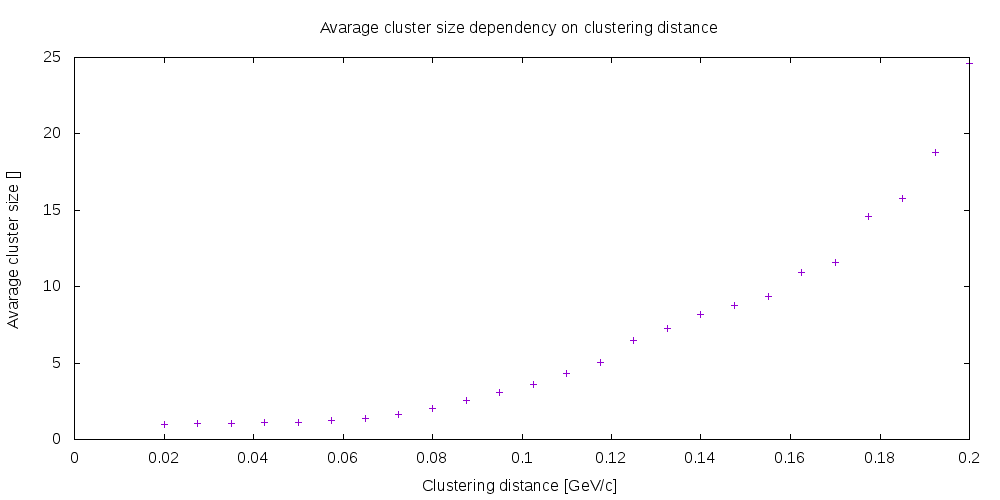
\includegraphics[width=0.94\textwidth]{../latex/momdist-mean.png}
\end{minipage}
\end{frame}

\begin{frame}[t]{Hivatkozások}
\begin{thebibliography}{9}
	\bibitem{CBMbook}
	Friman, Höhne, Knoll, Leupold, Randrup, Rapp, Senger
	\\\texttt{The CBM Physics Book - Compressed Baryonic Matter in Laboratory Experiments 2011 (Springer) Lect. Notes Phys.}
				
	\bibitem{phiALICE}
	 Tapia Takaki, J.D.
	 \\\texttt{ALICE Collaboration Journal of Physics G Nuclear Physics, 35, 044058 2008}
				
	\bibitem{CBMexp}
	 V.Vovchenko, I.Vassiliev, I.Kisel, M.Zyzak
	 \\\texttt{$\Phi$-meson production in Au+Au collisions and its feasibility in the CBM experiment, CBM Progress Report 2014}
				
	\bibitem{phiRICH}
	Bravina, L., Csernai, L., Faessler, A., et al. 2003, Nuclear Physics A, 715, 665 
				
	\bibitem{phiSTAR}
	F. Wang, R. Bossingham, Q. Li, I. Sakrejda,  N. Xu 
	\\\texttt{$\Phi$-meson reconstruction in the STAR TPC, 1998}
\end{thebibliography}
\end{frame}

\begin{frame}[t]{Hivatkozások}
\begin{thebibliography}{9}
	\bibitem{cbmFAIR}
	Hans Rudolf Schmidt
	\\\texttt{Hyperons at CBM-FAIR, Journal of Physics: Conference Series 736}
	
	\bibitem{challenges}
	The European Physics Journal A
	\\\texttt{Challenges in QCD matter physics - The scientific programme of the Compressed Baryonic Matter experiment at FAIR}
\end{thebibliography}
\end{frame}

\end{document}
